%% Segundo Avance del Proyecto, Electiva de Ingeniería de Software
%% USB Cali, plantilla elsarticle (preprint, 12pt)
\documentclass[preprint,12pt]{elsarticle}

\usepackage[utf8]{inputenc}
\usepackage[T1]{fontenc}
\usepackage[spanish,es-tabla]{babel}
\spanishdeactivate{<>}
\usepackage{amssymb}
\usepackage{amsmath}
\usepackage{graphicx}
\usepackage{booktabs}
\usepackage{array}
\usepackage{tikz}
\usetikzlibrary{arrows.meta,positioning}

\journal{Electiva de Ingeniería de Software, Universidad de San Buenaventura Cali}

\begin{document}

\begin{frontmatter}

\title{Segmentación Semántica Automática de Espacio Verde Urbano y Arbolado Mediante Aprendizaje Profundo Sobre Nubes de Puntos 3D}

\author{Julian David Fuentes Granja}
\affiliation{organization={Facultad de Ingeniería, Universidad de San Buenaventura Cali},
            city={Cali},
            country={Colombia}}

\begin{abstract}
El inventario del arbolado urbano con censos de campo es lento y costoso, y las imágenes aéreas 2D no capturan la estructura vertical de la copa. Este segundo avance formula el problema como un proceso de dos etapas, el aislamiento de cada árbol en la nube de puntos LiDAR aérea y la clasificación de su especie, y se concentra en la segunda etapa. El estado del arte se amplía con trabajos recientes sobre arquitecturas para nubes de puntos, segmentación de árboles individuales y clasificación de especies. El experimento usa el dataset público UrbanTree3D, con 152 árboles de seis especies, y compara PointNet, PointNet++ y DGCNN con un bosque aleatorio sobre descriptores geométricos bajo la partición oficial del dataset y tres semillas. Los resultados son preliminares porque el conjunto de prueba solo tiene 26 árboles y algunas especies cuentan con dos o tres ejemplares.
\end{abstract}

\begin{keyword}
Point Cloud \sep Deep Learning \sep Urban Forestry \sep Semantic Segmentation \sep LiDAR
\end{keyword}

\end{frontmatter}

\section{Definición del problema}
\label{sec:problema}

El inventario de la vegetación en las ciudades permite calcular métricas de salud ambiental, evaluar el riesgo de caída de árboles sobre vías e infraestructura eléctrica y gestionar los espacios verdes urbanos. Los árboles urbanos aportan servicios ecosistémicos como la regulación de la temperatura y la conservación de la biodiversidad \cite{fath2025urbantrees,jovanovic2025urbantrees}. Históricamente, el seguimiento se ha hecho con censos manuales en el terreno o con fotografías aéreas 2D. Las imágenes 2D sufren por las sombras proyectadas y no capturan el volumen, la copa ni la altura del árbol. El LiDAR aerotransportado resuelve esa limitación porque entrega la geometría tridimensional directa de la ciudad \cite{oshio2024mapping,dong2025highprecision}.

La entrada del sistema es una nube de puntos desordenada $P=\{p_1,\dots,p_n\}$, donde cada punto $p_i$ tiene coordenadas espaciales $(x_i,y_i,z_i)$ y atributos del sensor como la intensidad $I_i$.
\begin{equation}
P = \{p_i\}_{i=1}^{n}, \qquad p_i = (x_i, y_i, z_i, I_i).
\label{eq:pointcloud}
\end{equation}

El objetivo se descompone en dos etapas. La primera particiona la nube en $K$ árboles individuales y descarta el resto de la escena mediante una función de asignación $s$.
\begin{equation}
s : P \rightarrow \{0, 1, \dots, K\}, \qquad P_k = \{p_i \in P : s(p_i) = k\}, \quad k = 1, \dots, K,
\label{eq:instancias}
\end{equation}
donde $k=0$ representa el fondo, es decir suelo, edificios y otros objetos. La segunda etapa asigna una especie a cada árbol aislado mediante una red neuronal $f_\theta$ de parámetros $\theta$.
\begin{equation}
f_\theta : P_k \rightarrow \{1, \dots, C\}, \qquad C = 6.
\label{eq:clasificacion}
\end{equation}

El dataset elegido ya trae resuelta la primera etapa, porque sus autores aislaron cada árbol con DBSCAN y Watershed \cite{hamdani2026hybrid,hamdani2026urbantree3d}. Por eso el experimento de esta entrega se concentra en la ecuación~\eqref{eq:clasificacion}. Este alcance ajusta el planteamiento de la primera entrega, que hablaba de segmentación semántica a nivel de punto. UrbanTree3D tiene una etiqueta de especie por árbol, y por eso la clasificación del árbol completo es la tarea que el dataset permite evaluar con rigor. La segmentación por punto queda como trabajo futuro y exigiría anotar la escena completa.

\section{Estado del arte}
\label{sec:estado-arte}

\subsection{Arquitecturas de aprendizaje profundo sobre nubes de puntos}

El procesamiento de nubes de puntos pasó de convertir los datos a vóxeles o proyecciones 2D a operar directamente sobre conjuntos desordenados de puntos. Guo et al. organizaron esta evolución en una revisión de clasificación, detección y segmentación \cite{guo2021survey}. PointNet fue la primera red en aplicar un perceptrón compartido a cada punto y agregar el resultado con un máximo simétrico, lo que la hace invariante al orden de los puntos \cite{qi2017pointnet}. Su limitación es que no modela vecindarios locales. PointNet++ la corrigió con una jerarquía de agrupamientos que aplica PointNet de forma recursiva y combina escalas para tolerar densidades desiguales \cite{qi2017pointnetpp}. DGCNN propone la convolución de aristas EdgeConv sobre un grafo de vecinos que se recalcula en el espacio de características de cada capa \cite{wang2019dgcnn}.

Otras familias atacan la escala y la precisión. KPConv define convoluciones con puntos kernel posicionados en el espacio, con una variante deformable \cite{thomas2019kpconv}. RandLA-Net combina muestreo aleatorio con agregación local para segmentar nubes de millones de puntos \cite{hu2020randla}. Esta última está pensada para escenas completas y no para un árbol aislado con pocos cientos de puntos, y por eso no se incluye en el experimento. Point Transformer aplica autoatención vectorial a los vecindarios locales y obtuvo 70.4\,\% de mIoU en el Área 5 de S3DIS \cite{zhao2021pointtransformer}. PointNeXt mostró que gran parte de la ventaja de los modelos recientes viene de la estrategia de entrenamiento y del tamaño del modelo, pues el mismo PointNet++ pasó de 77.9\,\% a 86.1\,\% de exactitud global en ScanObjectNN solo con mejores aumentos y optimización \cite{qian2022pointnext}. Point Transformer V3 reemplaza la búsqueda exacta de vecinos por un orden serializado de los puntos y reporta una velocidad tres veces mayor y un consumo de memoria diez veces menor que su versión anterior \cite{wu2024ptv3}. Estos resultados sugieren que, con pocos datos, conviene partir de arquitecturas simples y bien entrenadas.

\subsection{LiDAR y arbolado urbano}

El LiDAR aéreo de alta precisión sigue siendo esencial en la silvicultura urbana, porque los productos globales de altura de dosel muestran limitaciones en contextos urbanos \cite{dong2025highprecision}. Oshio y Asawa mapearon la estructura 3D de árboles urbanos con LiDAR aéreo para levantamientos topográficos \cite{oshio2024mapping}. Yang et al. propusieron modelos para identificar la estructura vertical de la vegetación urbana con LiDAR de UAV \cite{yang2026vertical}, y Marks et al. mejoraron el LiDAR aéreo sobre paisajes vegetados mediante la fusión de imágenes SAR y ópticas con atención \cite{marks2025attention}.

Para aislar árboles individuales hay dos estrategias. Los métodos de agrupamiento y cuencas, como el DBSCAN \cite{ester1996dbscan} combinado con Watershed, delimitan las copas sin entrenamiento y son los que usó UrbanTree3D \cite{hamdani2026hybrid}. Los métodos de aprendizaje profundo de extremo a extremo, como ForestFormer3D, segmentan instancias de árboles en nubes forestales \cite{xiang2025forestformer3d}. Ruoppa et al. publicaron el benchmark FGI-EMIT para evaluar la segmentación de árboles individuales con LiDAR aéreo multiespectral \cite{ruoppa2025fgiemit}. Taher et al. observaron que los errores de segmentación degradan la clasificación posterior, pues repetir el benchmark solo con segmentos casi perfectos elevó la exactitud entre dos y tres puntos porcentuales \cite{taher2025msals}.

\subsection{Clasificación de especies con aprendizaje profundo}

Seidel et al. clasificaron siete especies con una CNN sobre imágenes 2D derivadas de nubes de puntos terrestres y alcanzaron cerca de 86\,\% de exactitud, mejor y más rápido que PointNet en su estudio \cite{seidel2021species}. Briechle et al. aplicaron PointNet++ a LiDAR de UAV y a imágenes multiespectrales para distinguir pino, abedul, aliso y árboles muertos en pie. Obtuvieron 90.2\,\% de exactitud global frente a 85.3\,\% de un bosque aleatorio con descriptores manuales \cite{briechle2020pointnetpp}.

Los benchmarks recientes comparan muchas arquitecturas. Taher et al. evaluaron 17 algoritmos de aprendizaje profundo y 9 de aprendizaje automático sobre LiDAR aéreo multiespectral, y el Point Transformer fue el de mayor exactitud \cite{taher2025msals}. Puliti et al. presentaron FOR-species20K, con más de 20\,000 árboles de 33 especies, y encontraron que los modelos basados en imágenes multivista alcanzaron una exactitud promedio de 0.77 frente a 0.72 de los modelos sobre nubes de puntos \cite{puliti2025forspecies}. Hamdani et al. compararon PointNet, DGCNN y RandLA-Net sobre LiDAR multiespectral de especies urbanas, y PointNet obtuvo la mejor exactitud global en prueba, con 82.07\,\% \cite{hamdani2026classification}. En un trabajo posterior optimizaron PointNet++ sobre FOR-species20K y, con 8\,192 puntos por árbol, lograron un F1 macro de 89.65\,\% sobre 508 árboles de prueba frente a 74.9\,\% reportado antes por Puliti et al. \cite{hamdani2026optimisation}. Estos números cambian con el dataset, el sensor y el número de especies, y por eso no se pueden comparar entre sí sin cuidado.

\subsection{Datasets y métricas}

La Tabla~\ref{tab:datasets} resume los datasets de árboles que aparecen en la literatura más cercana.

\begin{table}[h]
\centering
\footnotesize
\renewcommand{\arraystretch}{1.2}
\begin{tabular}{>{\raggedright\arraybackslash}p{2.7cm} >{\raggedright\arraybackslash}p{3.4cm} >{\raggedright\arraybackslash}p{2.4cm} >{\raggedright\arraybackslash}p{1.7cm} >{\raggedright\arraybackslash}p{3.3cm}}
\toprule
Dataset & Fuente & Escala & Especie & Limitación principal \\
\midrule
PureForest \cite{gaydon2024pureforest} & LiDAR aéreo y ortofoto & 449 áreas forestales & Sí & No separa árboles individuales \\
FOR-instance \cite{puliti2023forinstance} & LiDAR de UAV & 1\,130 árboles & No & Sin etiquetas de especie \\
FOR-species20K \cite{puliti2025forspecies} & TLS, MLS y UAV & Más de 20\,000 árboles & Sí & Densidad y adquisición heterogéneas \\
MS-ALS-SPECIES \cite{taher2025msals} & LiDAR aéreo multiespectral & 6\,326 árboles & Sí & Variabilidad ligada al sensor \\
StreetTree \cite{li2026streettree} & Imágenes RGB & 12 millones de árboles & Sí & Sin datos LiDAR 3D \\
UrbanTree3D \cite{hamdani2026urbantree3d} & LiDAR aéreo e inventario de campo & 152 árboles urbanos & Sí & Tamaño reducido \\
\bottomrule
\end{tabular}
\caption{Datasets de árboles en la literatura cercana. Las columnas de fuente, escala y limitación siguen la comparación del descriptor de datos de UrbanTree3D.}
\label{tab:datasets}
\end{table}

Las métricas habituales en clasificación de especies son la exactitud global, el F1 macro y la exactitud balanceada, y en segmentación el IoU medio. Con clases desbalanceadas, la exactitud global favorece a la especie mayoritaria, por lo que este trabajo reporta el F1 macro como métrica principal.

\subsection{Análisis comparativo y vacío que atiende la propuesta}

La revisión deja tres observaciones. Los resultados de mayor exactitud provienen de datasets grandes o multiespectrales \cite{taher2025msals,hamdani2026optimisation}, y hay pocas evaluaciones sobre árboles urbanos con LiDAR monoespectral y validación botánica en campo. Los trabajos sobre nubes de puntos suelen comparar arquitecturas profundas entre sí, y la comparación con descriptores geométricos clásicos es menos frecuente, aunque Briechle et al. muestran que el bosque aleatorio sigue siendo una referencia fuerte \cite{briechle2020pointnetpp}. El único estudio publicado con UrbanTree3D usa PointNet++ con 8\,192 puntos y reporta exactitud de validación \cite{hamdani2026urbantree3d}, sin comparar otras arquitecturas ni usar la métrica F1 macro en prueba.

Esta propuesta atiende ese vacío con un protocolo único sobre UrbanTree3D que enfrenta tres arquitecturas de puntos con un baseline clásico, con el mismo conjunto de prueba y tres semillas, y reporta el F1 macro de prueba. La Sección~\ref{sec:metodos} detalla el procedimiento.

\section{Materiales y métodos}
\label{sec:metodos}

\subsection{Selección y descripción del dataset}
\label{sec:dataset}

Se usa UrbanTree3D \cite{hamdani2026urbantree3d,hamdani2026zenodo}, publicado en la revista \textit{Data} (MDPI) y alojado en Zenodo. La Tabla~\ref{tab:ficha} presenta su ficha técnica. Las cifras de puntos por árbol y de altura se calcularon directamente sobre los archivos descargados.

\begin{table}[h]
\centering
\small
\begin{tabular}{>{\raggedright\arraybackslash}p{3.6cm} >{\raggedright\arraybackslash}p{10.2cm}}
\toprule
Campo & Descripción \\
\midrule
Nombre y DOI & UrbanTree3D, DOI 10.5281/zenodo.19475932 (descriptor en \textit{Data} 11(6), 147) \\
Origen & LiDAR aéreo de alta densidad del IGN de Francia e inventario de campo de la Communauté d'Agglomération Grand Paris Sud, con validación en terreno \\
Adquisición & LiDAR del 27 de enero de 2024 con al menos 10 pulsos por m$^2$, e inventario de septiembre de 2024 \\
Registros & 152 árboles individuales, un archivo LAS por árbol \\
Puntos por árbol & Entre 61 y 3\,739, con mediana de 429 y media de 847 \\
Altura de los árboles & Entre 3.1 y 16.8 m, con media de 8.9 m \\
Clases & 6 especies. \textit{Aesculus hippocastanum} (62), \textit{Prunus serrulata} (12), \textit{Pyrus calleryana} (15), \textit{Salix alba} (23), \textit{Tilia platyphyllos} (25) y \textit{Tilia $\times$ europaea} (15) \\
Atributos por punto & Coordenadas $X$, $Y$, $Z$ en Lambert-93, intensidad, número de retorno, clase ASPRS de vegetación (baja, media o alta) y tiempo GPS \\
Formato y tamaño & LAS 1.4, un archivo comprimido de 1.8 MB, más un archivo de metadatos y un archivo con la partición \\
Partición oficial & 104 árboles de entrenamiento, 22 de validación y 26 de prueba, estratificada por especie \\
Licencia y acceso & CC BY 4.0, acceso público sin registro \\
\bottomrule
\end{tabular}
\caption{Ficha técnica del dataset UrbanTree3D.}
\label{tab:ficha}
\end{table}

El dataset es urbano y sus etiquetas de especie fueron validadas por botánicos y verificadas en terreno. Tiene un descriptor en una revista indexada y una licencia abierta, y su tamaño permite entrenar y repetir experimentos en CPU en pocos minutos. El propio descriptor ya lo usó en un trabajo previo, con el que entrenó PointNet++ con 8\,192 puntos durante 105 épocas y reportó una exactitud de validación de 0.94 a 0.96 con aumento por rotación y de unos 0.87 sin aumento, con tres semillas \cite{hamdani2026urbantree3d}. Esa referencia permite una comparación cuantitativa directa sobre el mismo conjunto de validación. La limitación principal es el tamaño, ya que las clases minoritarias tienen entre 12 y 25 árboles y su conjunto de prueba contiene apenas dos o tres ejemplares de algunas especies.

\subsection{Preprocesamiento}

Las nubes ya vienen filtradas por los autores del dataset, que aplicaron remoción estadística de valores atípicos, normalización de altura con un modelo digital del terreno y segmentación de cada árbol \cite{hamdani2026urbantree3d}. Sobre esos archivos se aplica lo siguiente.

Para las redes de puntos, cada árbol se centra en su centroide y se escala a la esfera unitaria dividiendo entre la mayor distancia al centroide. Así la red recibe la forma del árbol y no su tamaño absoluto. Se muestrean 1\,024 puntos por árbol, con reemplazo cuando el árbol tiene menos puntos. En entrenamiento el muestreo se renueva en cada época. En validación y prueba se fija una sola muestra con una semilla constante, y todos los modelos ven exactamente los mismos puntos.

Durante el entrenamiento cada árbol se rota de forma aleatoria alrededor del eje vertical, se escala por eje con un factor entre 0.85 y 1.15, recibe un ruido gaussiano de desviación 0.01 y pierde hasta 20\,\% de sus puntos de forma aleatoria. El descriptor del dataset recomienda aplicar el aumento solo al conjunto de entrenamiento, y así se hizo.

\subsection{Arquitecturas}

Se implementaron tres redes en PyTorch, que se muestran en la Figura~\ref{fig:arq}. Todas reciben 1\,024 puntos con coordenadas $(x,y,z)$ y producen seis logits.

\begin{figure}[h]
\centering
\resizebox{\textwidth}{!}{%
\begin{tikzpicture}[
  font=\footnotesize,
  caja/.style={draw, rounded corners=2pt, minimum height=0.95cm, minimum width=1.9cm, align=center, fill=blue!7},
  glob/.style={draw, rounded corners=2pt, minimum height=0.95cm, minimum width=1.9cm, align=center, fill=orange!15},
  sal/.style={draw, rounded corners=2pt, minimum height=0.95cm, minimum width=1.9cm, align=center, fill=green!12},
  flecha/.style={-{Stealth[length=2mm]}, thick}
]
\node[font=\bfseries, anchor=west] at (-1,2.6) {PointNet};
\node[caja] (a0) at (0,1.6) {Entrada\\$1024\times 3$};
\node[caja, right=0.4cm of a0] (a1) {MLP\\64, 128, 1024};
\node[glob, right=0.4cm of a1] (a2) {Máximo\\global};
\node[caja, right=0.4cm of a2] (a3) {FC\\512, 256};
\node[sal, right=0.4cm of a3] (a4) {Logits\\6};
\foreach \i/\j in {a0/a1,a1/a2,a2/a3,a3/a4} \draw[flecha] (\i) -- (\j);

\node[font=\bfseries, anchor=west] at (-1,0.45) {PointNet++};
\node[caja] (b0) at (0,-0.55) {Entrada\\$1024\times 3$};
\node[caja, right=0.4cm of b0] (b1) {SA1\\256 centros\\$r=0.2$, 32 vec.};
\node[caja, right=0.4cm of b1] (b2) {SA2\\64 centros\\$r=0.4$, 32 vec.};
\node[glob, right=0.4cm of b2] (b3) {MLP 256, 512,\\1024 y máximo};
\node[caja, right=0.4cm of b3] (b4) {FC\\512, 256};
\node[sal, right=0.4cm of b4] (b5) {Logits\\6};
\foreach \i/\j in {b0/b1,b1/b2,b2/b3,b3/b4,b4/b5} \draw[flecha] (\i) -- (\j);

\node[font=\bfseries, anchor=west] at (-1,-1.7) {DGCNN};
\node[caja] (c0) at (0,-2.7) {Entrada\\$1024\times 3$};
\node[caja, right=0.4cm of c0] (c1) {EdgeConv\\64, $k=16$};
\node[caja, right=0.4cm of c1] (c2) {EdgeConv\\64, $k=16$};
\node[caja, right=0.4cm of c2] (c3) {EdgeConv\\128, $k=16$};
\node[glob, right=0.4cm of c3] (c4) {Conv 1024,\\máximo y media};
\node[caja, right=0.4cm of c4] (c5) {FC\\512, 256};
\node[sal, right=0.4cm of c5] (c6) {Logits\\6};
\foreach \i/\j in {c0/c1,c1/c2,c2/c3,c3/c4,c4/c5,c5/c6} \draw[flecha] (\i) -- (\j);
\end{tikzpicture}}
\caption{Arquitecturas comparadas. SA es una capa de abstracción de conjuntos, FC una capa totalmente conectada y $r$ el radio de agrupamiento.}
\label{fig:arq}
\end{figure}

\paragraph{PointNet}
Un perceptrón compartido por punto, implementado con convoluciones de tamaño 1, transforma las coordenadas con capas de 64, 128 y 1\,024 canales, cada una con normalización por lote y ReLU. Un máximo sobre los puntos produce un vector global de 1\,024 valores. Una cabeza con capas de 512 y 256 unidades, normalización por lote, ReLU y \textit{dropout} de 0.4 produce los seis logits. No incluye las redes de transformación espacial de la versión original. Tiene 0.80 millones de parámetros.

\paragraph{PointNet++}
Se usa la variante de agrupamiento de una sola escala. La primera capa de abstracción elige 256 centros con muestreo del punto más lejano y agrupa 32 vecinos dentro de un radio de 0.2, con un perceptrón de 64, 64 y 128 canales. La segunda elige 64 centros con radio 0.4 y 32 vecinos, con un perceptrón de 128, 128 y 256 canales. Una capa global con 256, 512 y 1\,024 canales y un máximo producen el vector que recibe la misma cabeza de clasificación de PointNet. Tiene 1.46 millones de parámetros.

\paragraph{DGCNN}
Tres capas EdgeConv sucesivas con 64, 64 y 128 canales construyen un grafo de $k=16$ vecinos más cercanos en el espacio de características de cada capa, y la agregación toma el máximo sobre los vecinos. Después de cada convolución se aplica normalización por lote y LeakyReLU con pendiente 0.2. Las tres salidas se concatenan en 256 canales y se proyectan a 1\,024 con una convolución de tamaño 1. La concatenación del máximo y la media globales, de 2\,048 valores, alimenta la cabeza de 512 y 256 unidades con \textit{dropout} de 0.4. Tiene 1.47 millones de parámetros.

\paragraph{Baseline clásico}
Es un bosque aleatorio \cite{breiman2001rf} de 500 árboles con pesos de clase balanceados, entrenado sobre descriptores calculados de cada nube completa. Hay dos variantes. La variante sin escala usa 27 descriptores independientes del tamaño, que son los percentiles de altura normalizada, un histograma vertical de diez cajas, los tres valores propios normalizados de la covarianza, la media y la desviación del radio de copa, la relación entre los anchos horizontales, la media y la desviación de la altura normalizada, y la media y la desviación de la intensidad y de los retornos. La variante con escala agrega la altura, el ancho de copa, su relación y el logaritmo del número de puntos, para un total de 31 descriptores. Este baseline usa la intensidad y los retornos del LiDAR, que las redes de puntos no reciben, y esa diferencia se discute en la Sección~\ref{sec:discusion}.

\subsection{Protocolo de entrenamiento}

Las tres redes se entrenan con entropía cruzada ponderada, donde el peso de la especie $c$ es la raíz cuadrada de la razón entre el promedio de ejemplos por clase y los ejemplos de esa clase en entrenamiento.
\begin{equation}
\mathcal{L}(\theta) = -\frac{1}{B}\sum_{b=1}^{B} w_{y_b}\,\log \hat{p}_\theta\!\left(y_b \mid P_b\right), \qquad w_c = \sqrt{\frac{n}{C\,n_c}},
\label{eq:loss}
\end{equation}
donde $B$ es el tamaño del lote, $n$ el total de árboles de entrenamiento y $n_c$ los de la especie $c$. Se usa el optimizador Adam \cite{kingma2015adam} con tasa de aprendizaje inicial de $10^{-3}$, decaimiento de pesos de $10^{-4}$, un programa de coseno a lo largo de 60 épocas y lotes de 16 árboles. En cada época se evalúa el F1 macro de validación y se conserva el modelo con el mejor valor, con la exactitud de validación como criterio de desempate. Los experimentos se repiten con las semillas 0, 5 y 95, las mismas del descriptor del dataset, y se mantiene fija la partición oficial. El entrenamiento se ejecutó en CPU con PyTorch 2.12 y Python 3.13.

\subsection{Protocolo de evaluación}

Las métricas se calculan sobre los 26 árboles de prueba a partir de la matriz de confusión $M$, donde $M_{ij}$ cuenta los árboles de la especie $i$ predichos como $j$.
\begin{equation}
\mathrm{Exactitud} = \frac{\sum_c M_{cc}}{\sum_{i,j} M_{ij}}, \qquad F_{1,c} = \frac{2\,M_{cc}}{\sum_j M_{cj} + \sum_i M_{ic}}, \qquad F_{1}^{\text{macro}} = \frac{1}{C}\sum_{c=1}^{C} F_{1,c}.
\label{eq:metrics}
\end{equation}
La exactitud balanceada es el promedio de la exhaustividad por clase. Se reporta la media y la desviación estándar muestral de las tres semillas. El conjunto de validación solo se usa para elegir la época y no para comparar métodos en el texto principal, salvo en la comparación con el descriptor del dataset. El código y las tablas se pueden reproducir con los archivos entregados, que descargan los datos desde su DOI.

\section{Resultados preliminares}
\label{sec:resultados}

La Tabla~\ref{tab:principal} resume el desempeño de los cinco métodos sobre los 26 árboles de prueba. PointNet obtuvo el mayor F1 macro, con 0.919, seguido por el bosque aleatorio sin escala con 0.906, DGCNN con 0.896, el bosque aleatorio con escala con 0.864 y PointNet++ con 0.844. En exactitud, PointNet y el bosque aleatorio sin escala empatan en 0.910. Con 26 árboles, un solo error equivale a 3.8 puntos porcentuales de exactitud, y por eso las diferencias entre PointNet, DGCNN y el bosque aleatorio sin escala no superan lo que cambiaría un árbol. PointNet++ tuvo la mayor variación entre semillas, con exactitudes de prueba de 0.769, 0.885 y 0.923.

\begin{table}[h]
\centering
\footnotesize
\resizebox{\textwidth}{!}{%
\begin{tabular}{lcccccc}
\toprule
Método & Exact. prueba & F1 macro prueba & Exact. balanc. prueba & Exact. validación & F1 macro validación & Parám. (M) \\
\midrule
RF con escala & 0.872 $\pm$ 0.022 & 0.864 $\pm$ 0.023 & 0.872 $\pm$ 0.024 & 0.864 $\pm$ 0.000 & 0.821 $\pm$ 0.014 & -- \\
RF sin escala & 0.910 $\pm$ 0.022 & 0.906 $\pm$ 0.016 & 0.922 $\pm$ 0.010 & 0.833 $\pm$ 0.026 & 0.813 $\pm$ 0.033 & -- \\
PointNet & 0.910 $\pm$ 0.022 & 0.919 $\pm$ 0.030 & 0.923 $\pm$ 0.032 & 1.000 $\pm$ 0.000 & 1.000 $\pm$ 0.000 & 0.80 \\
PointNet++ & 0.859 $\pm$ 0.080 & 0.844 $\pm$ 0.102 & 0.866 $\pm$ 0.093 & 0.909 $\pm$ 0.045 & 0.864 $\pm$ 0.063 & 1.46 \\
DGCNN & 0.897 $\pm$ 0.022 & 0.896 $\pm$ 0.012 & 0.921 $\pm$ 0.018 & 0.985 $\pm$ 0.026 & 0.978 $\pm$ 0.038 & 1.47 \\
\bottomrule

\end{tabular}}
\caption{Resultados con media y desviación estándar muestral de tres semillas. Las métricas de prueba usan 26 árboles y las de validación 22. Los parámetros se dan en millones.}
\label{tab:principal}
\end{table}

La Tabla~\ref{tab:clases} muestra el F1 por especie en el conjunto de prueba. \textit{Prunus serrulata} y \textit{Tilia platyphyllos} se clasifican casi sin errores con PointNet, mientras que \textit{Tilia $\times$ europaea} resulta la especie más difícil para PointNet++, con un F1 de 0.67. La especie con más árboles, \textit{Aesculus hippocastanum}, obtiene un F1 de 0.90 a 0.93 con todos los métodos.

\begin{table}[h]
\centering
\footnotesize
\resizebox{\textwidth}{!}{%
\begin{tabular}{lcccccc}
\toprule
Método & \textit{A. hippocastanum} & \textit{P. serrulata} & \textit{P. calleryana} & \textit{S. alba} & \textit{T. platyphyllos} & \textit{T. $\times$ europaea} \\
\midrule
RF con escala & 0.92 & 1.00 & 0.71 & 0.90 & 0.80 & 0.86 \\
RF sin escala & 0.93 & 1.00 & 0.80 & 0.96 & 0.89 & 0.86 \\
PointNet & 0.90 & 1.00 & 0.89 & 0.86 & 1.00 & 0.87 \\
PointNet++ & 0.91 & 0.93 & 0.80 & 0.88 & 0.87 & 0.67 \\
DGCNN & 0.91 & 0.93 & 0.82 & 0.90 & 0.92 & 0.90 \\
\bottomrule

\end{tabular}}
\caption{F1 por especie en el conjunto de prueba, promedio de tres semillas.}
\label{tab:clases}
\end{table}

La Figura~\ref{fig:confusion} presenta la matriz de confusión de PointNet, la red con mejor F1 de validación, sumada sobre las tres semillas. De los 78 casos de prueba, 71 se clasificaron bien. Tres de los siete errores son árboles de \textit{Salix alba} predichos como \textit{Aesculus hippocastanum}, dos son \textit{Aesculus hippocastanum} predichos como \textit{Tilia $\times$ europaea}, uno es \textit{Aesculus hippocastanum} predicho como \textit{Pyrus calleryana} y uno es \textit{Pyrus calleryana} predicho como \textit{Tilia $\times$ europaea}. En las tres redes, el error más repetido fue \textit{Aesculus hippocastanum} predicho como \textit{Tilia $\times$ europaea}, con dos o tres casos por red.

\begin{figure}[h]
\centering
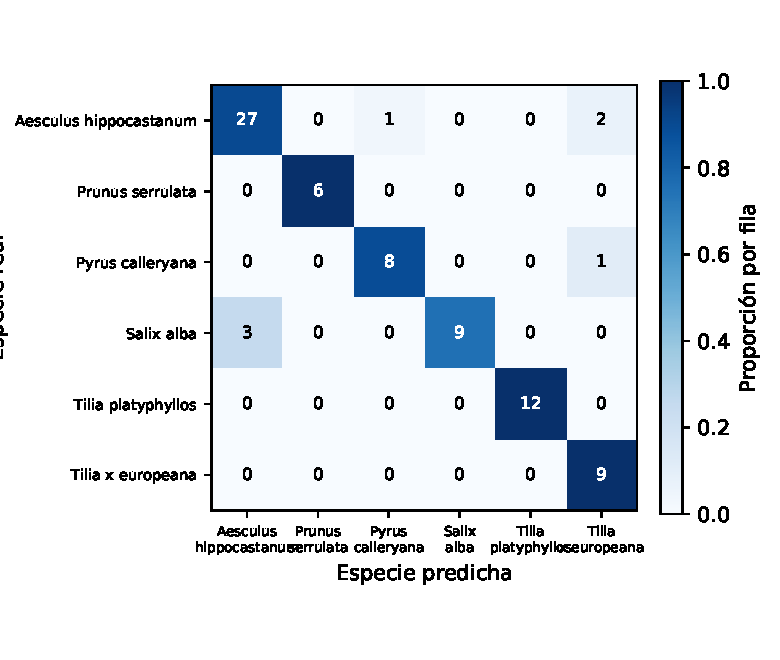
\includegraphics[width=0.6\textwidth]{figuras/confusion.pdf}
\caption{Matriz de confusión de PointNet en el conjunto de prueba, con los conteos sumados de las tres semillas.}
\label{fig:confusion}
\end{figure}

La Figura~\ref{fig:cualitativo} muestra un árbol de prueba por especie con las predicciones de PointNet y del bosque aleatorio sin escala de la semilla 0. Cada método falla en un árbol distinto, lo que indica que sus errores no coinciden del todo. Las vistas laterales también muestran que algunas nubes incluyen puntos que no son del árbol, como una banda horizontal cerca del suelo en el ejemplo de \textit{Prunus serrulata}.

\begin{figure}[h]
\centering
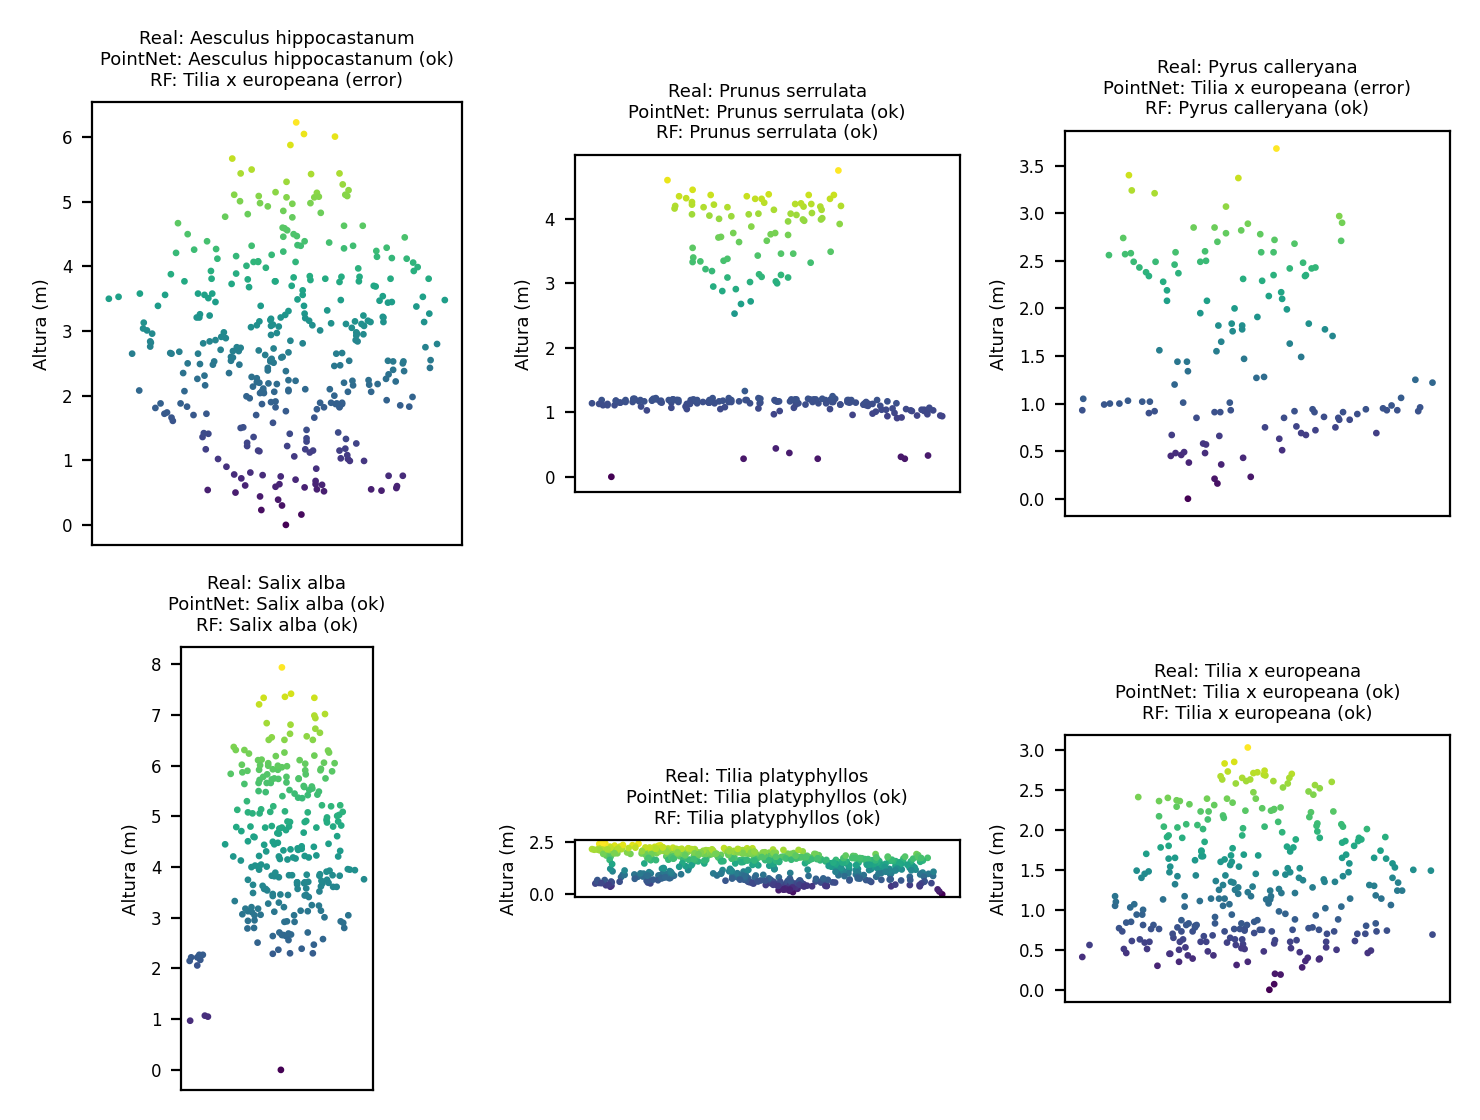
\includegraphics[width=0.9\textwidth]{figuras/cualitativo.png}
\caption{Vista lateral de un árbol de prueba por especie, coloreado por altura, con la especie real y las predicciones de PointNet y del bosque aleatorio sin escala.}
\label{fig:cualitativo}
\end{figure}

La Figura~\ref{fig:curvas} muestra la evolución del entrenamiento de la semilla 0. Las tres redes reducen la pérdida de forma estable, y el F1 de validación de PointNet++ sube más despacio que el de las otras dos. En una prueba aislada de dos épocas, PointNet tardó 4.1 segundos, PointNet++ 7.9 y DGCNN 20.6 segundos en CPU. Los tiempos de los entrenamientos completos no se comparan porque se ejecutaron en paralelo y compitieron por el mismo procesador.

\begin{figure}[h]
\centering
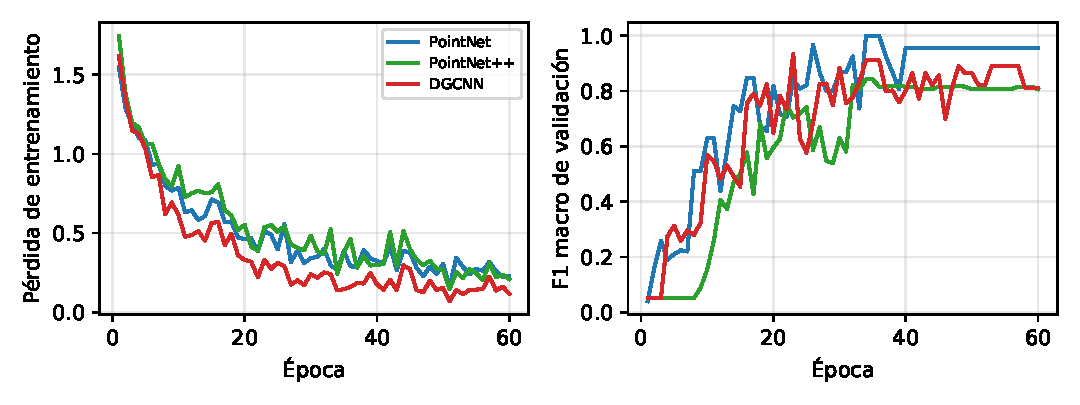
\includegraphics[width=0.9\textwidth]{figuras/curvas.pdf}
\caption{Pérdida de entrenamiento y F1 macro de validación por época, semilla 0.}
\label{fig:curvas}
\end{figure}

\section{Discusión}
\label{sec:discusion}

Los resultados muestran que tres redes de puntos y un bosque aleatorio alcanzan entre 0.86 y 0.91 de exactitud sobre este conjunto de prueba, y que el tamaño del conjunto no permite declarar un ganador. La diferencia entre el mejor y el cuarto método equivale a menos de dos árboles. PointNet, la arquitectura más simple, no queda por debajo de DGCNN ni de PointNet++. Esto es coherente con lo que reportan Qian et al., para quienes la estrategia de entrenamiento pesa tanto como la arquitectura \cite{qian2022pointnext}, y con que Hamdani et al. encontraron que PointNet superó a DGCNN y a RandLA-Net en otro dataset urbano \cite{hamdani2026classification}.

La exactitud de validación de PointNet++ fue de 0.909 con 1\,024 puntos, por debajo del rango de 0.94 a 0.96 que reporta el descriptor del dataset con 8\,192 puntos y aumento por rotación \cite{hamdani2026urbantree3d}. La comparación no es exacta, porque el número de puntos, el número de épocas y la implementación difieren, y porque aquí el conjunto de validación también se usó para elegir la época, lo que infla esa cifra, sobre todo el 1.000 de PointNet. La diferencia es compatible con que 1\,024 puntos describan peor la copa que 8\,192, y esa es la primera variable que conviene probar. Los errores principales también coinciden con los del descriptor, que señala la confusión entre \textit{Aesculus hippocastanum} y \textit{Tilia $\times$ europaea} por su copa de tamaño y densidad parecidos.

El bosque aleatorio es un baseline fuerte, como ya había mostrado Briechle et al. frente a PointNet++ \cite{briechle2020pointnetpp}. La variante sin escala superó a la variante con escala, y por eso agregar la altura, el ancho de copa y el número de puntos no ayudó en este conjunto. Una explicación posible es que el número de puntos dependa de la posición del árbol respecto a la trayectoria del sensor y no de la especie, aunque esta hipótesis no se comprobó. El bosque aleatorio también recibe la intensidad y los retornos del LiDAR, que las redes no reciben, y por eso la comparación favorece a este baseline y no mide solo la geometría.

Las limitaciones son cuatro. El conjunto de prueba tiene 26 árboles y solo dos o tres ejemplares de algunas especies, por lo que cada F1 por especie es muy inestable. Se usó una única partición, sin validación cruzada, y las tres semillas solo varían la inicialización y los aumentos. Algunas nubes contienen puntos ajenos al árbol, lo que puede ayudar o perjudicar la clasificación según la especie. El experimento cubre solo la clasificación del árbol aislado y no evalúa la segmentación de instancias ni la segmentación por punto planteadas en la Sección~\ref{sec:problema}.

\section*{Conclusiones}

Este avance formalizó el problema como un proceso de aislamiento y clasificación de árboles, amplió el estado del arte con trabajos recientes sobre arquitecturas, datasets y métricas, y describió un protocolo experimental reproducible sobre UrbanTree3D. Con la partición oficial del dataset, PointNet, DGCNN y un bosque aleatorio alcanzaron resultados similares, con F1 macro de prueba entre 0.90 y 0.92, y PointNet++ quedó más abajo y con mayor variación. El tamaño del conjunto de prueba impide afirmar que alguno sea mejor.

El trabajo pendiente tiene cuatro pasos. El primero es aumentar el número de puntos por árbol a 8\,192 para comparar con el descriptor del dataset. El segundo es repetir el protocolo con validación cruzada estratificada para reducir la incertidumbre de la prueba. El tercero es dar la intensidad y los retornos como entrada a las redes, para igualar la información del baseline. El cuarto es probar una arquitectura más reciente, como PointNeXt o Point Transformer V3, y evaluar la segmentación de la escena completa con un dataset que tenga anotación por punto.

\bibliographystyle{elsarticle-num}
\bibliography{referencias}

\end{document}
